\documentclass[notes,11pt, aspectratio=169]{beamer}

\usepackage{pgfpages}
% These slides also contain speaker notes. You can print just the slides,
% just the notes, or both, depending on the setting below. Comment out the want
% you want.
\setbeameroption{hide notes} % Only slide
%\setbeameroption{show only notes} % Only notes
%\setbeameroption{show notes on second screen=right} % Both

\usepackage{helvet}
\usepackage[default]{lato}
\usepackage{array}
\usepackage{tgbonum}

\usepackage{tikz}
\usepackage{verbatim}
\setbeamertemplate{note page}{\pagecolor{yellow!5}\insertnote}
\usetikzlibrary{positioning}
\usetikzlibrary{snakes}
\usetikzlibrary{calc}
\usetikzlibrary{arrows}
\usetikzlibrary{decorations.markings}
\usetikzlibrary{shapes.misc}
\usetikzlibrary{matrix,shapes,arrows,fit,tikzmark}
\usepackage{amsmath}
\usepackage{mathpazo}
\usepackage{hyperref}
\usepackage{lipsum}
\usepackage{multimedia}
\usepackage{graphicx}
\usepackage{multirow}
\usepackage{graphicx}
\usepackage{dcolumn}
\usepackage{bbm}
\newcolumntype{d}[0]{D{.}{.}{5}}

\usepackage{changepage}
\usepackage{appendixnumberbeamer}
\newcommand{\beginbackup}{
   \newcounter{framenumbervorappendix}
   \setcounter{framenumbervorappendix}{\value{framenumber}}
   \setbeamertemplate{footline}
   {
     \leavevmode%
     \hline
     box{%
       \begin{beamercolorbox}[wd=\paperwidth,ht=2.25ex,dp=1ex,right]{footlinecolor}%
%         \insertframenumber  \hspace*{2ex} 
       \end{beamercolorbox}}%
     \vskip0pt%
   }
 }
\newcommand{\backupend}{
   \addtocounter{framenumbervorappendix}{-\value{framenumber}}
   \addtocounter{framenumber}{\value{framenumbervorappendix}} 
}


\usepackage{graphicx}
\usepackage[space]{grffile}
\usepackage{booktabs}
\newcommand\independent{\protect\mathpalette{\protect\independenT}{\perp}}
\def\independenT#1#2{\mathrel{\rlap{$#1#2$}\mkern2mu{#1#2}}}
\DeclareMathOperator{\Supp}{Supp}

% These are my colors -- there are many like them, but these ones are mine.
\definecolor{blue}{RGB}{0,114,178}
\definecolor{red}{RGB}{213,94,0}
\definecolor{yellow}{RGB}{240,228,66}
\definecolor{green}{RGB}{0,158,115}

\hypersetup{
  colorlinks=false,
  linkbordercolor = {white},
  linkcolor = {blue}
}


%% I use a beige off white for my background
\definecolor{MyBackground}{RGB}{255,253,218}

%% Uncomment this if you want to change the background color to something else
%\setbeamercolor{background canvas}{bg=MyBackground}

%% Change the bg color to adjust your transition slide background color!
\newenvironment{transitionframe}{
  \setbeamercolor{background canvas}{bg=yellow}
  \begin{frame}}{
    \end{frame}
}

\setbeamercolor{frametitle}{fg=blue}
\setbeamercolor{title}{fg=black}
\setbeamertemplate{footline}[frame number]
\setbeamertemplate{navigation symbols}{} 
\setbeamertemplate{itemize items}{-}
\setbeamercolor{itemize item}{fg=blue}
\setbeamercolor{itemize subitem}{fg=blue}
\setbeamercolor{enumerate item}{fg=blue}
\setbeamercolor{enumerate subitem}{fg=blue}
\setbeamercolor{button}{bg=MyBackground,fg=blue,}



% If you like road maps, rather than having clutter at the top, have a roadmap show up at the end of each section 
% (and after your introduction)
% Uncomment this is if you want the roadmap!
% \AtBeginSection[]
% {
%    \begin{frame}
%        \frametitle{Roadmap of Talk}
%        \tableofcontents[currentsection]
%    \end{frame}
% }
\setbeamercolor{section in toc}{fg=blue}
\setbeamercolor{subsection in toc}{fg=red}
\setbeamersize{text margin left=1em,text margin right=1em} 

\newenvironment{wideitemize}{\itemize\addtolength{\itemsep}{10pt}}{\enditemize}

\usepackage{environ}
\NewEnviron{videoframe}[1]{
  \begin{frame}
    \vspace{-8pt}
    \begin{columns}[onlytextwidth, T] % align columns
      \begin{column}{.70\textwidth}
        \begin{minipage}[t][\textheight][t]
          {\dimexpr\textwidth}
          \vspace{8pt}
          \hspace{4pt} {\Large \sc \textcolor{blue}{#1}}
          \vspace{8pt}
          
          \BODY
        \end{minipage}
      \end{column}%
      \hfill%
      \begin{column}{.38\textwidth}
        \colorbox{green!20}{\begin{minipage}[t][1.2\textheight][t]
            {\dimexpr\textwidth}
            Face goes here
          \end{minipage}}
      \end{column}%
    \end{columns}
  \end{frame}
}

\title[]{\textcolor{blue}{Linear Regression IV: Penalized Regression Models }}
\author[PGP]{}
\institute[FRBNY]{\small{Paul Goldsmith-Pinkham}}
\date{\today}


\begin{document}

%%% TIKZ STUFF
\tikzset{   
        every picture/.style={remember picture,baseline},
        every node/.style={anchor=base,align=center,outer sep=1.5pt},
        every path/.style={thick},
        }
\newcommand\marktopleft[1]{%
    \tikz[overlay,remember picture] 
        \node (marker-#1-a) at (-.3em,.3em) {};%
}
\newcommand\markbottomright[2]{%
    \tikz[overlay,remember picture] 
        \node (marker-#1-b) at (0em,0em) {};%
}
\tikzstyle{every picture}+=[remember picture] 
\tikzstyle{mybox} =[draw=black, very thick, rectangle, inner sep=10pt, inner ysep=20pt]
\tikzstyle{fancytitle} =[draw=black,fill=red, text=white]
%%%% END TIKZ STUFF

% Title Slide
\begin{frame}
\maketitle

\end{frame}


\begin{frame}{Today's topic - penalized regression, e.g. Lasso}
  \begin{columns}[T] % align columns
    \begin{column}{.8\textwidth}
      \begin{wideitemize}
      \item Today: Machine learning methods of a particular kind
      \item Specifically, we will be focus on linear models that use
        penalization to select relevant right hand side variables
      \item Will mainly focus on Lasso (Least Absolute Shrinkage and
        Selection Operator ), coined by Tibshiriani in 1996
      \item Key concept underlying these methods -- \emph{model selection}
        \begin{itemize}
        \item This is typically not a topic great for causal inference
        \end{itemize}
      \item Ends up being very valuable in causal estimation!
        \begin{itemize}
        \item In select circumstances
        \end{itemize}
      \end{wideitemize}
    \end{column}%
  \hfill%
  \begin{column}{.5\textwidth}
  \end{column}
\end{columns}
\end{frame}


\begin{frame}{What's the big idea?}
  \begin{wideitemize}
  \item There are many circumstances when we have a problem like the following:
    \begin{enumerate}
    \item Many variables (too many) that we would like to use as regressors
    \item A unknown and potentially complicated function of many variables
    \end{enumerate}
  \item Two simple versions of this, in a setting where we have data
    $(Y_{i}, X_{i})$, and the dimension of $X_{i}$ is $p$
    \begin{enumerate}
    \item $Y_{i} = X_{i,0}\beta_{0} + \epsilon_{i},$ where $X_{i,0}$ is a
      vector of $p_{0} \leq p$ covariates, but you don't
      know which variables in your data $X_{i}$ are $X_{i,0}$. 
    \item $Y_{i} = f(X_{i}) + \epsilon_{i},$, and we want to
      approximate $f$ as best we can --- we can do complicated
      functions of $X_{i}$ to approximate it (a la semiparametrics)
      but this gets hard when $p$ grows.
    \end{enumerate}
    \item A key idea which will come up in our later results is
      \emph{sparsity} -- e.g. $p_{0}$ is small, or for $f$ that is can
      be approximated by a small number of variables (combinations of
      $X$)
  \end{wideitemize}
\end{frame}

\begin{frame}{What is Lasso? Tibshiriani (1996)}
  \begin{wideitemize}
  \item What is Lasso?  Let's stay in our simple linear model , and
    ignore issues of endogeneity
  \item Recall that the ``true'' model (which we prespecified) had only a subset of non-zero entries
    \begin{itemize}
    \item E.g., there are irrelevant regressors
    \item We would like to know which are the true right ones for purposes of interpretation
    \end{itemize}
  \item As our dataset grows, if $p$ stays fixed, OLS will eventually
    figure out which $\beta$ are zeros
    \begin{itemize}
    \item But it's not immediate -- only in the limit do the
      (``wrong'') estimates converge to zero!
    \item Worse yet, if the variables are correlated or noisy, it's
      hard to get good estimates that don't make the model poorly fit!
    \end{itemize}
  \item In finite samples, we would like to have an approach that
    selects the ``right'' variables to focus on , and fits the outcome well
    \begin{itemize}
    \item This is a model selection problem
    \item It's \emph{also} a regularization problem
    \end{itemize}
  \end{wideitemize}
\end{frame}

\begin{frame}{What is Lasso? Tibshiriani (1996)}
  \begin{wideitemize}
  \item Tibshiriani (1996) proposed Lasso to do both things -- identify the
    non-zero covariates and shrink estimates accordingly
  \item Let's compare OLS and Lasso's objective functions:
        \begin{align*}
      \min_{\beta} \; & n^{-1}\sum_{i=1}^{n}(Y_{i} - X_{i}\beta)^{2}   \;& \text{(OLS)}\\
      \min_{\beta} \;& n^{-1}\sum_{i=1}^{n}(Y_{i} - X_{i}\beta)^{2} + \lambda \sum_{k=1}^{p}|\beta_{k}|   \;& \text{(Lasso)}     \end{align*}
  \item In essence, Lasso added one ``thresholding'' penalty, where
    $\lambda$ is a tuning parameter chosen by the researcher.
  \item Lasso will choose to push coefficient values down to minimize objective 
    \begin{itemize}
    \item Most importantly, due to the $L_{1}$ norm, this will tend to push coefficients to \emph{zero}
    \item Why? Intuitively, if it was worth decreasing $\beta_{k}$
      slightly, it will continue to be worthwhile until it hits zero
    \end{itemize}
  \end{wideitemize}
\end{frame}

\begin{frame}{What is Lasso? Graphically}
  \begin{columns}[T] % align columns
    \begin{column}{.35\textwidth}
      \begin{wideitemize}
      \item Note that the first term in the  minimization
        $$n^{-1}\sum_{i=1}^{n}(Y_{i} - X_{i}\beta)^{2}$$
        is equivalent to
        $$(\beta- \beta_{ols})'X'X(\beta- \beta_{ols}) + C$$
      \item Hence given a $\lambda$ constraint we're finding the
        isoquant closest to $\beta_{ols}$
      \end{wideitemize}
    \end{column}%
  \hfill%
  \begin{column}{.65\textwidth}
    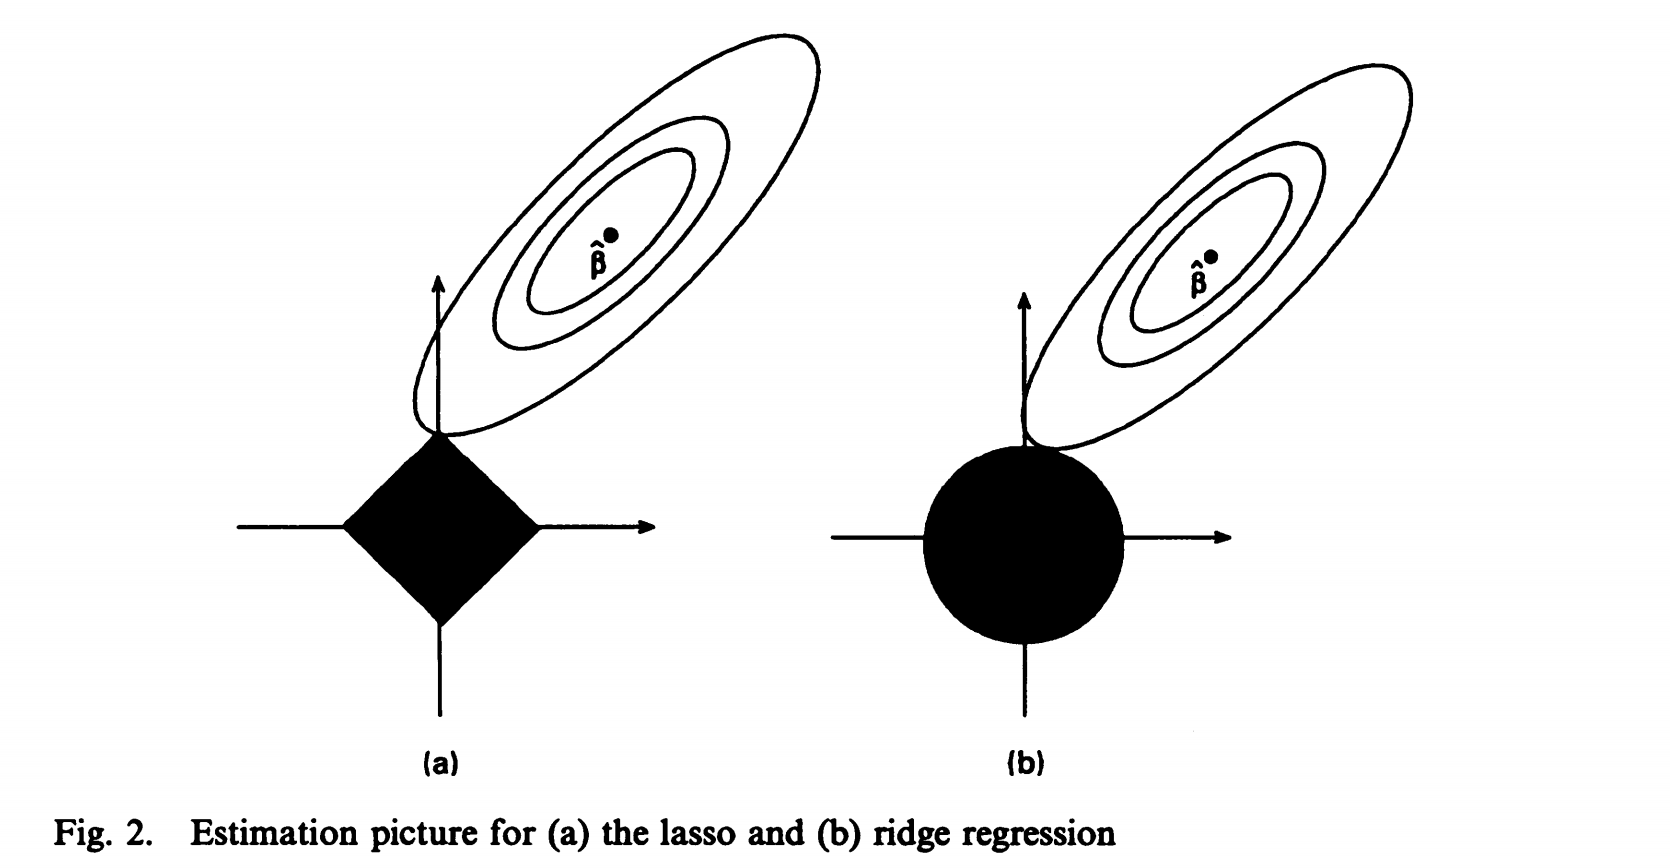
\includegraphics[width=\linewidth]{images/tibshiriani.png}
  \end{column}
\end{columns}
\end{frame}


\begin{frame}{What's so great about Lasso? A quick aside on MSE}
  \begin{wideitemize}
  \item Well, it (and modified versions of it) have two very nice properties:
    \begin{itemize}
    \item very efficient estimators -- they predict $Y$ well
    \item pick a subet of covariates, making model interpretation easier! 
    \end{itemize}
  \item A quick aside on regularized estimators. Recall that for a
    given estimator $\hat{\theta}$ of $\theta$, we care a lot about
    the mean squared error, $MSE(\hat{\theta})$, especially for predictors
    \begin{itemize}
    \item Recall that  $MSE(\hat{\theta}) = Var(\hat{\theta}) + Bias(\hat{\theta}, \theta)^{2}$
    \item In most estimation, we've cared a \emph{lot} about Bias being zero (or being small!)
    \item Regularized estimators give up a little bit of bias in order
      to reduce overall MSE
    \end{itemize}
  \item So a nice feature of Lasso is that is has lower MSE than OLS
    in most cases, but the terms can be biased
    \begin{itemize}
    \item This is true of ML approaches generally
    \end{itemize}
  \end{wideitemize}
\end{frame}


\begin{frame}{The magical Oracle property of Lasso}
  \begin{columns}[T] % align columns
    \begin{column}{.5\textwidth}
  \begin{wideitemize}
  \item One particularly interesting property of Lasso (and derivative
    approaches) is that it has what is called the ``oracle property''
    under certain conditions
  \item In essence, we get the ``right'' model and asymptotic
    normality!
  \item Your reaction may be ``this seems too good to be true''
    \begin{itemize}
    \item Don't worry, it is
    \item But it still does well!
    \end{itemize}
  \end{wideitemize}
    \end{column}%
  \hfill%
  \begin{column}{.5\textwidth}
    Zou (2006):
    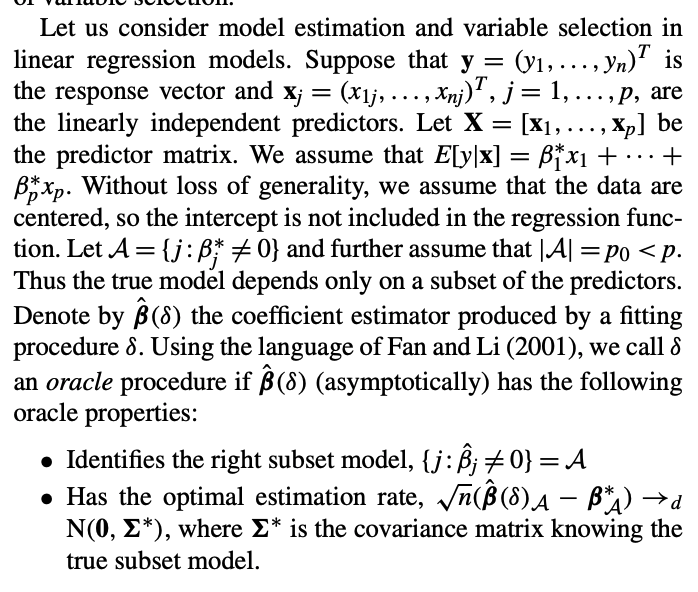
\includegraphics[width=\linewidth]{images/oracle_property.png}
  \end{column}
\end{columns}
\end{frame}

\begin{frame}{An aside on Pointwise vs. Uniform convergence}
  \begin{wideitemize}
    \item Recall that all our asymptotic results are about approximations to finite sample distributions
    \item In fact, Penalized and ML methods improve finite sample performance!
      \begin{itemize}
      \item OLS does very well with infeasibly \textbf{infinite} data
      \end{itemize}
    \item Recall from your econometrics courses the
      \emph{pointwise} convergence of an estimator
      \begin{itemize}
      \item Given a true estimand $\theta_{0}$, we can consider the
        convergence of $\hat{\theta}$ to that $\theta_{0}$
      \end{itemize}
    \item But, this holds fixed our value of $\theta_{0}$ -- we
      typically want \emph{uniform} convergence
      \begin{itemize}
      \item E.g. the convergence can be done across all values of
        $\theta_{0}$ simultaneously
      \end{itemize}
    \item Why does this matter? Uniform convergence matters for
      our asymptotic approximations to do a good job in approximating
      finite samples
  \end{wideitemize}
\end{frame}

\begin{frame}{Leeb and Potscher (2008)}
  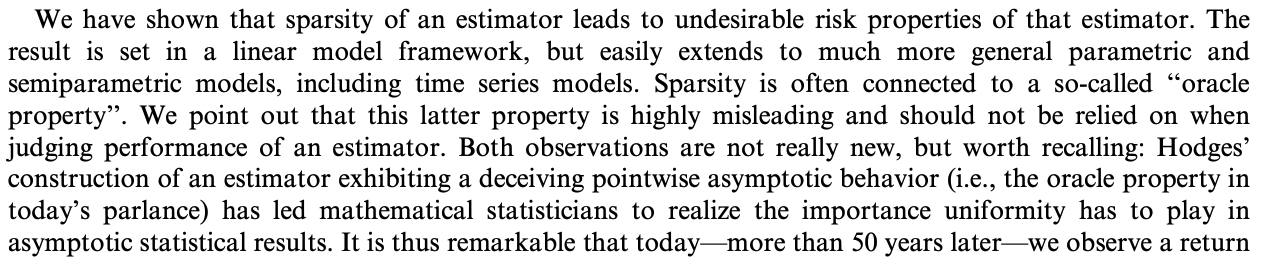
\includegraphics[width=\linewidth]{images/leebpotscher2.png}\\
  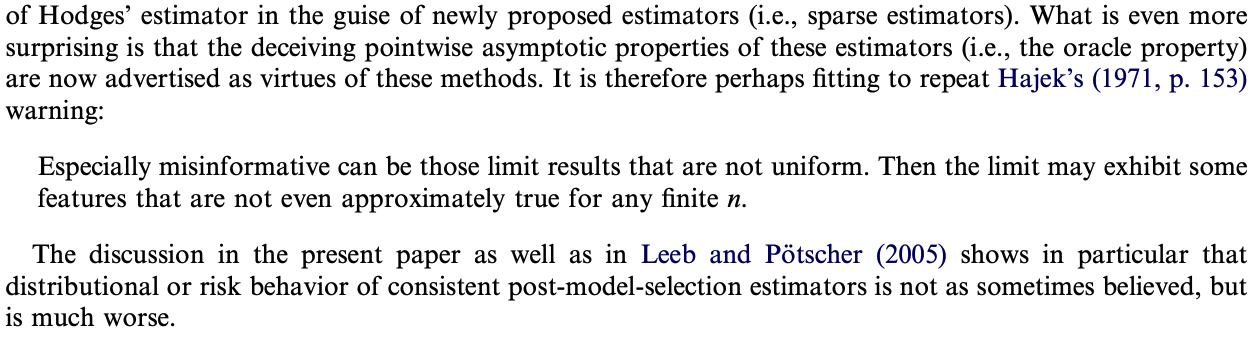
\includegraphics[width=\linewidth]{images/leebpotscher3.png}
\end{frame}

\begin{frame}{Back to lasso's  oracle property}
  \begin{columns}[T] % align columns
    \begin{column}{.8\textwidth}
      \begin{wideitemize}
      \item Leeb and Potscher (2005, 2008) say:  ``Wait, hold on.'' (They are much punchier than that)
      \item The implication is that we should not rely heavily on the
        oracle property of Lasso (and other penalized methods).
      \item This ability to select elements can be misleading
      \item This is not a new fact, and one that econometricians/statisticians should have been aware of
        \begin{itemize}
        \item E.g. Hodges' Estimator
        \end{itemize}
      \end{wideitemize}
    \end{column}%
  \hfill%
  \begin{column}{.5\textwidth}
  \end{column}
\end{columns}
\end{frame}


\begin{frame}{Example with Hodges' Estimator}
  \begin{columns}[T] % align columns
    \begin{column}{.6\textwidth}
      \begin{wideitemize}
      \item Consider an estimator $\hat{\theta}_{n}$ for $\theta$. Now we construct our new estimator,
        \begin{itemize}
        \item $\hat{\theta}_{n,hodge} = \hat{\theta}_{n}$ if $|\hat{\theta}_{n}|  \geq n^{-1/4}$
        \item $\hat{\theta}_{n,hodge} = 0$ if $|\hat{\theta}_{n}|  < n^{-1/4}$          
        \end{itemize}
      \item This is a quasi-shrunk estimator, with superefficient
        convergence of the estimator when $\theta = 0$ and normal
        asymptotic convergence everywhere else
      \item But, the convergence is not uniform, and creates very weird properties near zero
        \begin{itemize}
        \item Blue = $n=5$, purple = $n=50$, olive = $n=500$
        \end{itemize}
      \end{wideitemize}
    \end{column}%
  \hfill%
  \begin{column}{.4\textwidth}
    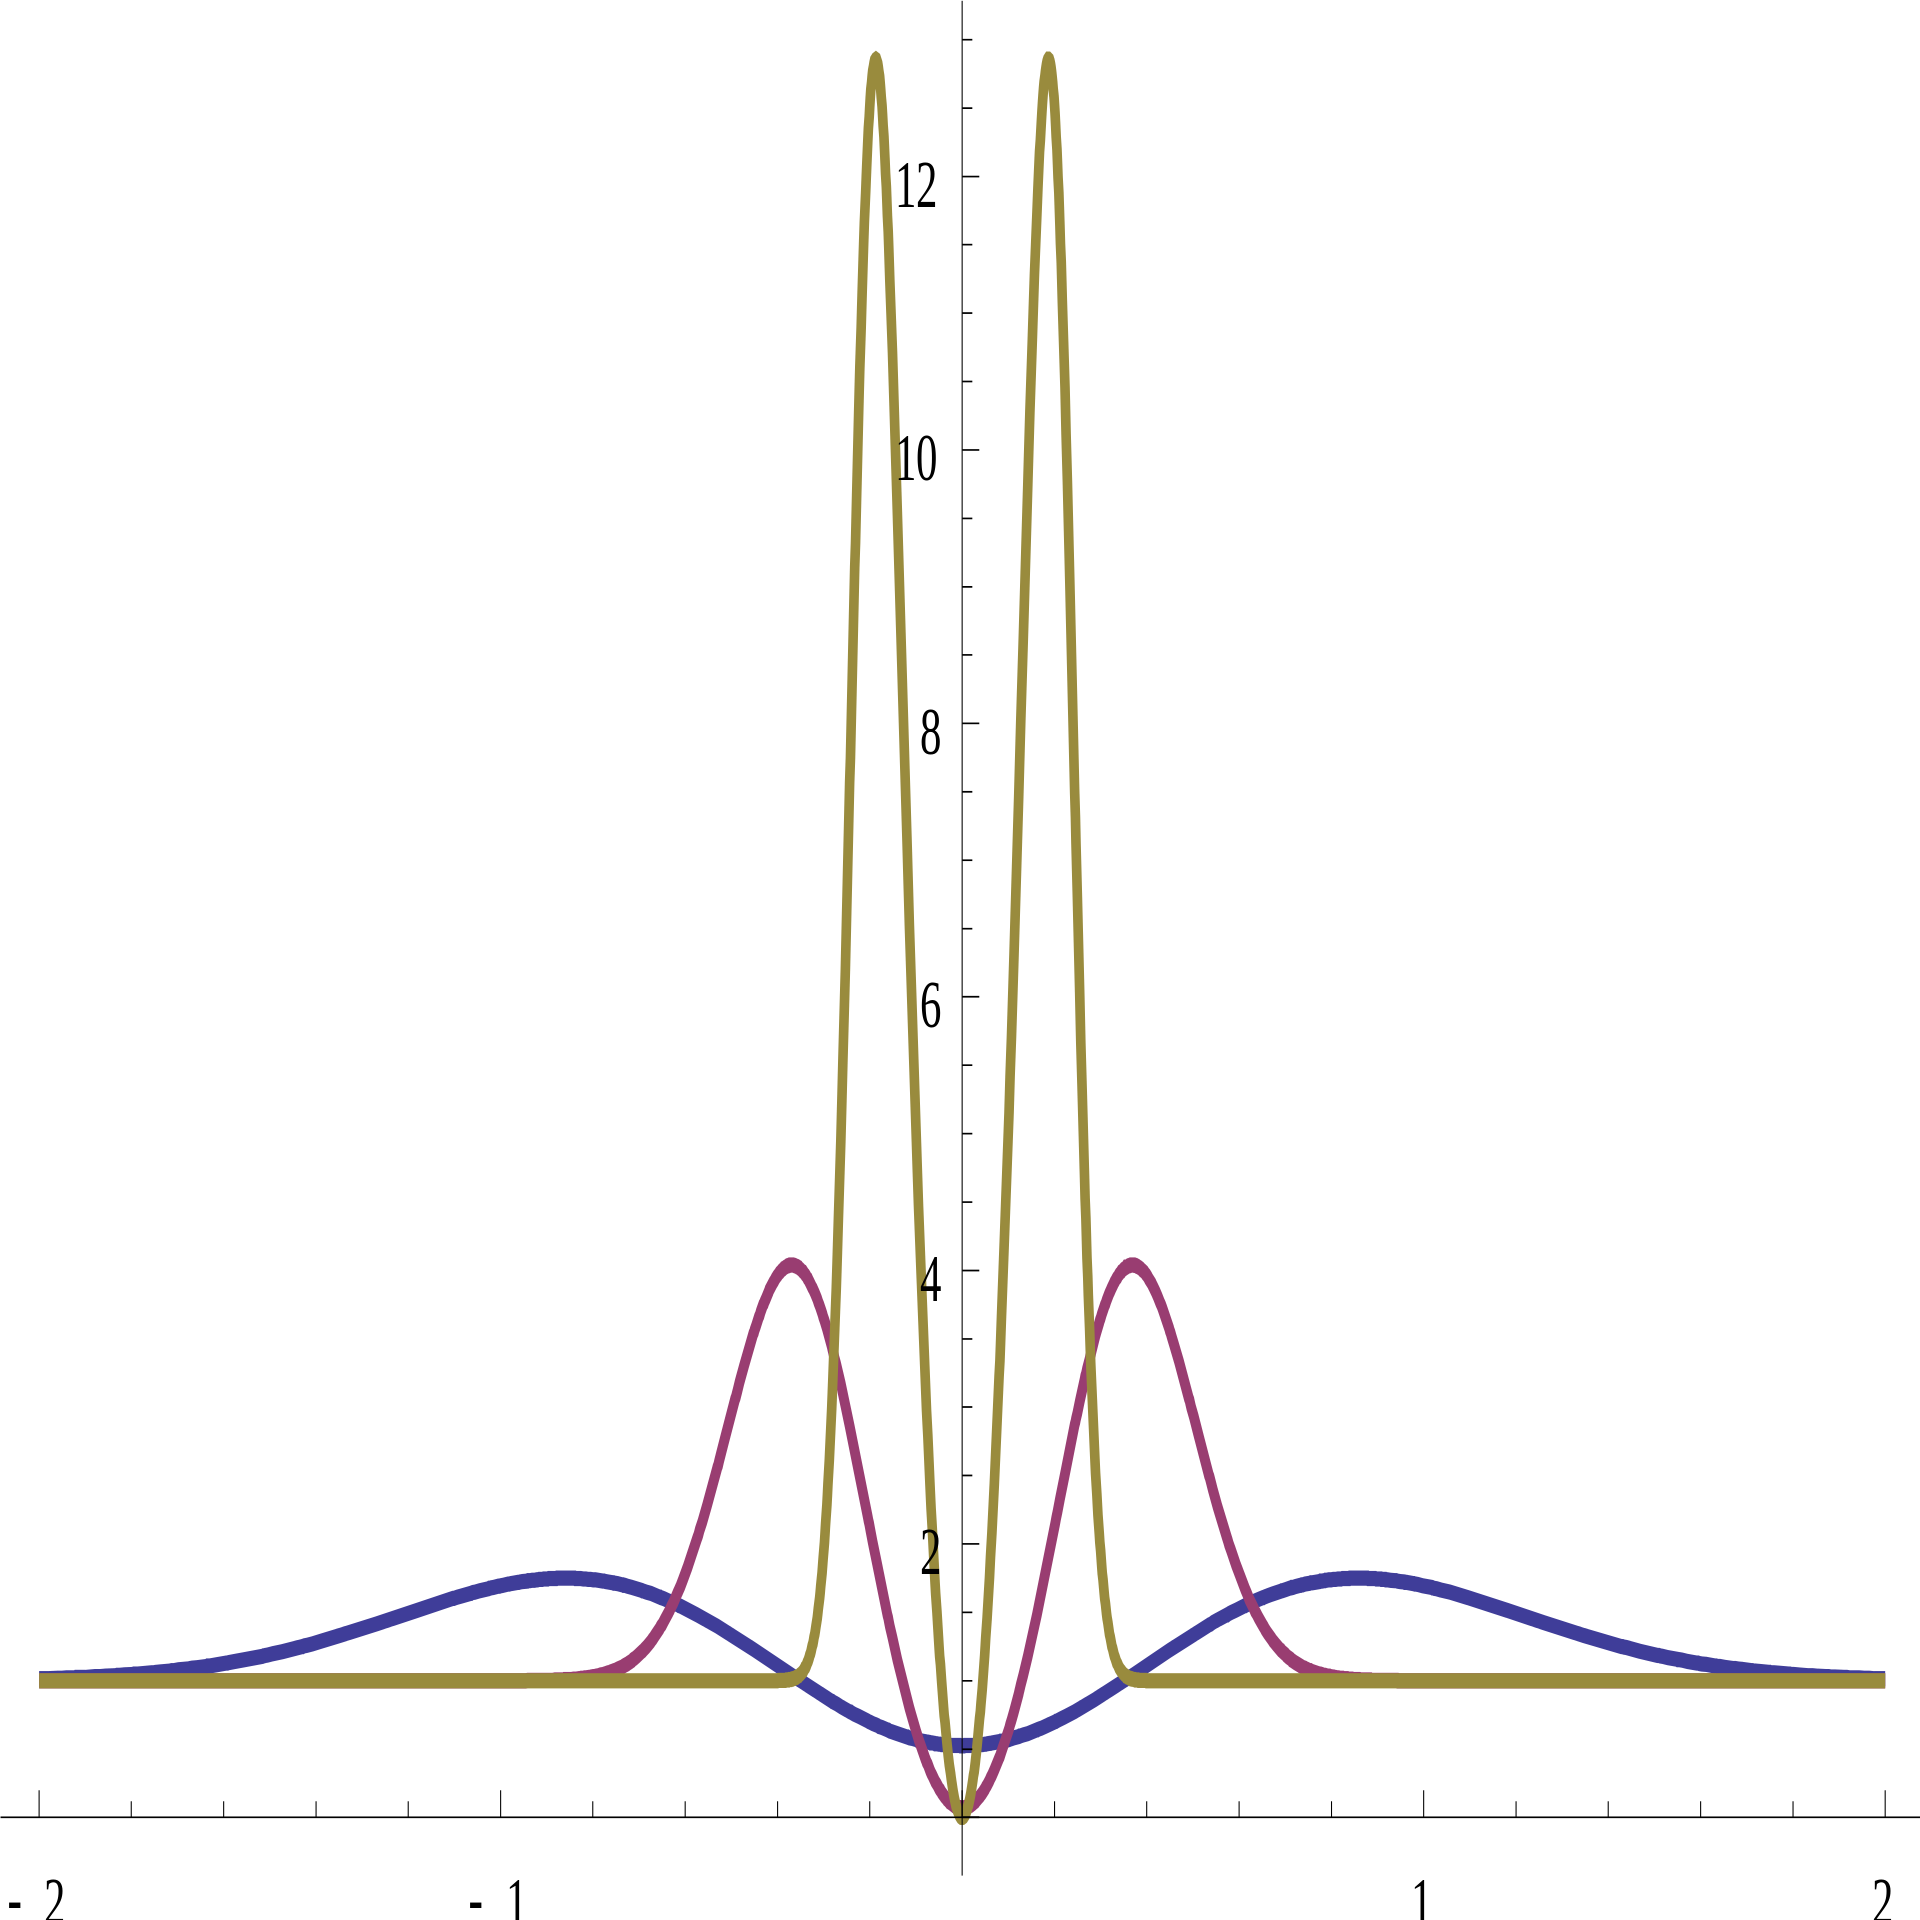
\includegraphics[width=\linewidth]{images/hodges.png}
  \end{column}
\end{columns}
\end{frame}

\begin{frame}{Irrepresentability}
  \begin{wideitemize}
  \item Important note -- the convergence results for Lasso hold under
    an important condition known as the irrepresentability condition.
  \item Many regressions have collinear regressors, as this is a
    natural feature of lots of statistical problems
  \item One very awkward property of Lasso is that having right-hand
    side variables that are highly correlated can create very weird
    problems
  \item If the covariates that should be excluded are correlated with
    the relevant covariates in a meaningful way, then it's possible
    that lasso will pick the irrelevant covariate, even for large
    sample
  \item This problem is very solveable -- simply orthogonalize the covariates manually!
    \begin{itemize}
    \item But that kind of defeats the ``interpretability'' point...
    \item But this is fixable!
    \end{itemize}
  \end{wideitemize}
\end{frame}

\begin{frame}{Puffer Transformation (Jia and Rohe (2015))}
  \begin{wideitemize}
  \item Key insight in linear model is that for a given $n \times n$ matrix $F$, we can premultiply and estimate
    $$FY = FX\beta + F\epsilon \qquad \text{vs.} \qquad Y = X\beta + \epsilon  $$
  \item Notatbly this will give us the $\beta$. However, if we use the
    appropriate tranformation (preconditioning) matrix, we can ensure
    that the consistency of the estimates hold
  \item Let $F = UD^{-1}U'$ be the Puffer transformation, where $U$
    and $D$ come from the Singular Value Decomposition of $X = UDV'$.
    \begin{itemize}
    \item Under this transformation, we can ensure consistent
      estimates of $\beta$, and most important, it's the \emph{same} $\beta$
    \item If we had orthogonalized our $X$, we woudl have a different
      linear combination of the underlying $\beta$
    \end{itemize}
  \item The tradeoff with this method is it can increase variance of
    the estimators. See the paper for details on implementation
  \end{wideitemize}
\end{frame}

\begin{frame}{The Geometry of Puffer}
\begin{center}
  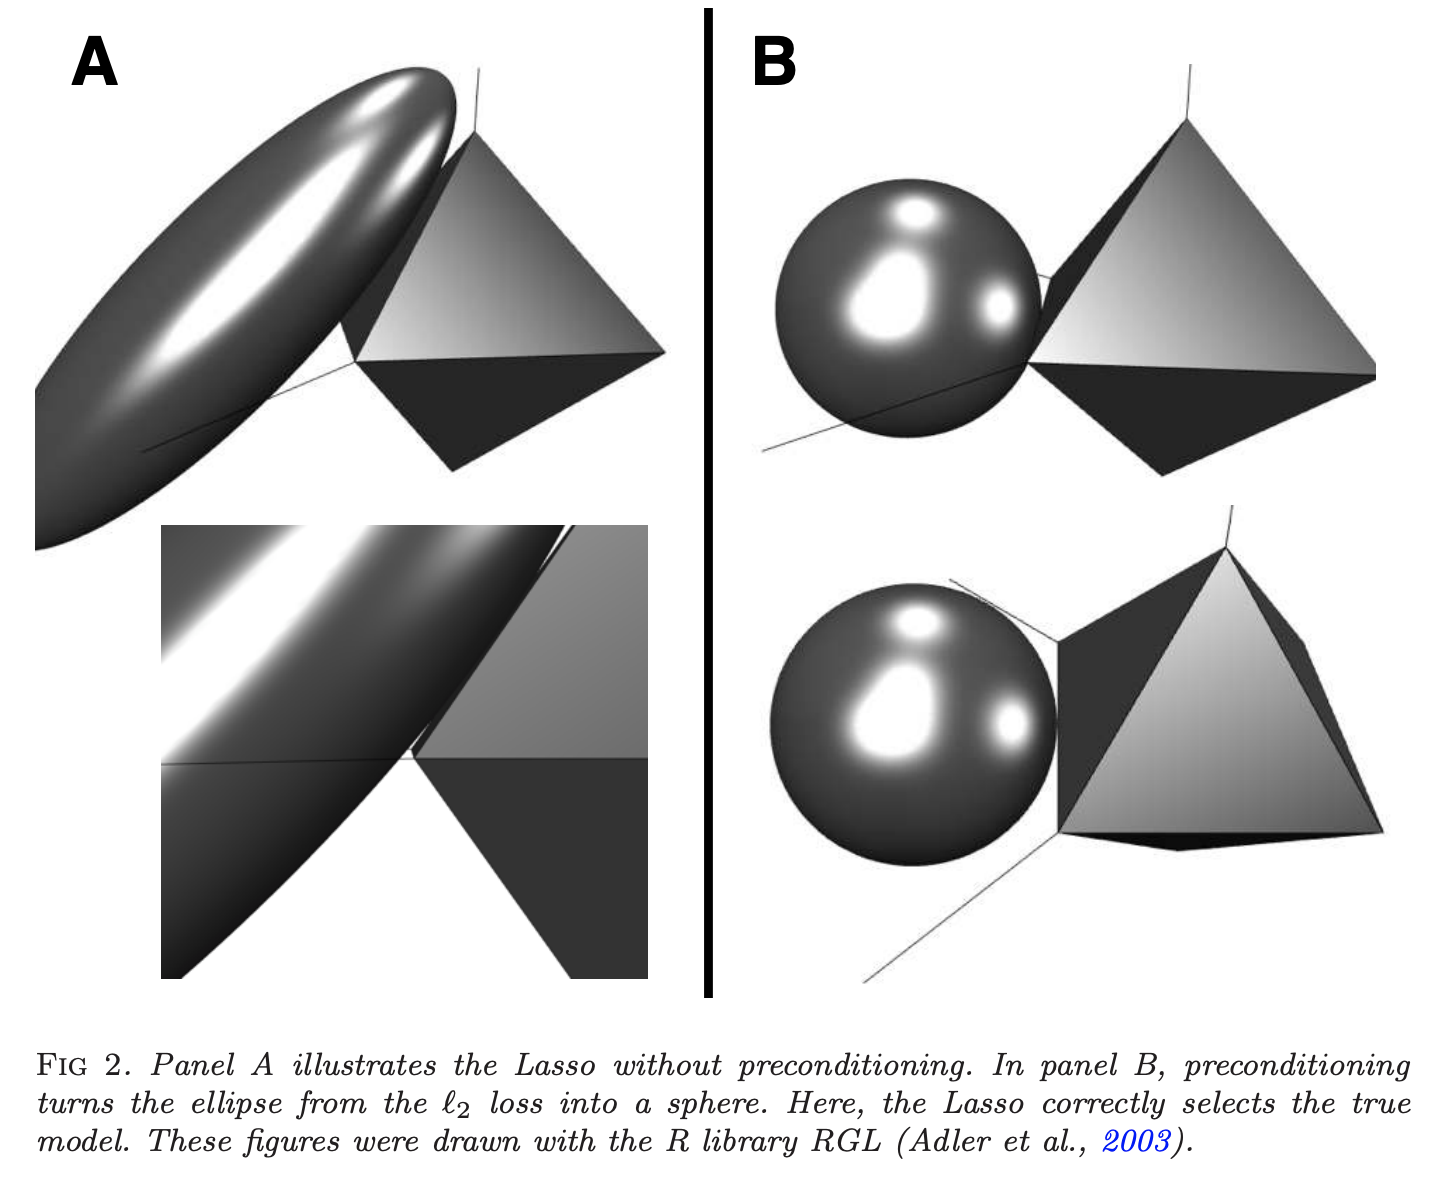
\includegraphics[width=0.65\linewidth]{images/puffer.png}
\end{center}
\end{frame}

\begin{frame}{Punchline for Lasso}
  \begin{wideitemize}
  \item Remember, asymptotics are approximations. Uniformity matters a
    lot! The thresholding criterion for Lasso creates weird behavior
    that can be unsmooth
  \item E.g. there's no free lunch!
  \item Or \emph{is} there?? Key point that we will revisit shortly --
    Lasso wanted to find all effects, no matter how small. What if we
    relax this?
    \begin{itemize}
    \item E.g., what if our goal is not the parameters themselves, but
      to approximate something in a way that does not create issues?
    \end{itemize}
  \end{wideitemize}
\end{frame}

\begin{frame}{Generalizations + Sparsity}
  \begin{columns}[T] % align columns
    \begin{column}{.7\textwidth}
      \begin{wideitemize}
      \item There are a number of other types of linear regularization methods
        \begin{itemize}
        \item We'll cover more non-linear methods later in the course
        \end{itemize}
      \item These include Ridge regression, Group Lasso, Elastic Net, Others
      \item These all revolve around methods to shrink with either L1 or
        L2 norms
        \begin{itemize}
        \item Many are dealing with highly correlated regressors
        \end{itemize}
      \item Today, will continue to focus on Lasso, which has been a major
        focus on econometrics research
        \begin{itemize}
        \item Why? Model selection aspect of Lasso + Sparsity assumption is very powerful
        \end{itemize}
      \end{wideitemize}
    \end{column}
  \hfill%
  \begin{column}{.3\textwidth}
    Other Linear Methods:
    \begin{itemize}
    \item Ridge Regression
    \item Elastic Net
    \item Group Lasso
    \item Fused Lasso
    \item Adaptive Lasso
    \item Bridge regression
    \item Bayesian Lasso
      \item Prior Lasso
      \end{itemize}
  \end{column}
\end{columns}
\end{frame}

\begin{frame}{So what? How does an applied economist use this?}
  \begin{wideitemize}
  \item   With that under our belt, let's discuss applications.
  \item Most direct historical purposes have been for prediction
    \begin{itemize}
    \item Prediction is extremely useful! 
    \end{itemize}
  \item Mullanaithan and Spiess (2017) discuss various uses of general ML
    \begin{itemize}
    \item Prediction in decision problems, e.g. bail decisions (or
      lending, Fuster, Goldsmith-Pinkham, Ramadorai and Walther
      (2020))
    \item Prediction in forecasting -- e.g. asset pricing. (For example, see Feng, Giglio and Xiu)
    \item Testing a model or predictor -- e.g. creating an ML
      benchmark 
    \end{itemize}
  \item What we'll discuss rest of today: how Lasso methods can be
    used in causal inference
  \end{wideitemize}
\end{frame}

\begin{frame}{Lasso and Nuisance Parameters}
    \begin{columns}[T] % align columns
    \begin{column}{.8\textwidth}
  \begin{wideitemize}
  \item Concise way to remember the relative merits of LASSO/ML
    vs. standard model: $\hat{y}$ vs $\hat{\beta}$ (Mullanaithan and
    Spiess (2017))
    \begin{itemize}
    \item Lasso is best for constructing a lower MSE estimate of
      something.
    \item You shouldn't always trust it for particular estimates of
      all the underlying parameters in the model (and inference can be 
      challenging for all of them without sparsity assumptions)
    \end{itemize}
  \item Remember the problem of semiparametric models and nuisance
    parameters? Turns out this is a great problem for us to solve!
    \begin{itemize}
    \item We have a function we need to estimate
    \item We don't care about the parameters of the function per se
    \end{itemize}
  \end{wideitemize}
\end{column}
\begin{column}{.3\textwidth}
  \begin{center}
    Lasso     vs.    OLS
$$\hat{y} \;\; \text{vs.} \;\; \hat{\beta}$$
    \end{center}
  \end{column}
\end{columns}

\end{frame}

\begin{frame}{Partial linear model}
  \begin{wideitemize}
  \item Consider a partially additive model:
    $$Y_{i} = D_{i}\tau + g_{0}(X_{i}) + U_{i}$$
    where $D_{i}$ is randomly assigned, and $X$ are pre-treatment covariates , and $g_{0}$ is some unknown function.
  \item A simpler version of this could be
    $$Y_{i} = D_{i}\tau + X_{i,0}\beta + U_{i}$$
    where we don't know which $X_{i}$ are in the model
  \item Note that the estimation of $g_{0}$ (or the $\beta$) are
    \emph{nuisance} parameters -- we'd like them to get good / better
    estimates of $\tau$, but we don't care about them \emph{per se}
  \end{wideitemize}
\end{frame}

\begin{frame}{Partial linear model and causal inference}
  \begin{wideitemize}
  \item There are a lot of results in this space, heavily influenced
    by Victor Chernozhukov.
    
  \item  Going to touch on two points:
  \begin{enumerate}
  \item How did they address the Leeb and Potscher issue
  \item How to address the bias variance problem if interested in causal parameters?
  \end{enumerate}
\item Many of the insights here carry over into the linear IV case
  \begin{itemize}
  \item Today, we'll focus on exogeneous regressors (e.g. random
    experiment)
  \end{itemize}
\item This discussion riffs heavily on Chernozhukov, Chetverikov,
  Demirer, Duflo, Hansen, Newey and Robins (2017,2018) and Belloni,
  Chernozhukov, and Hansen (2014)
  \end{wideitemize}
\end{frame}

\begin{frame}{Why would we need ML if RCT?}
  Regarding ML and RCTs:
  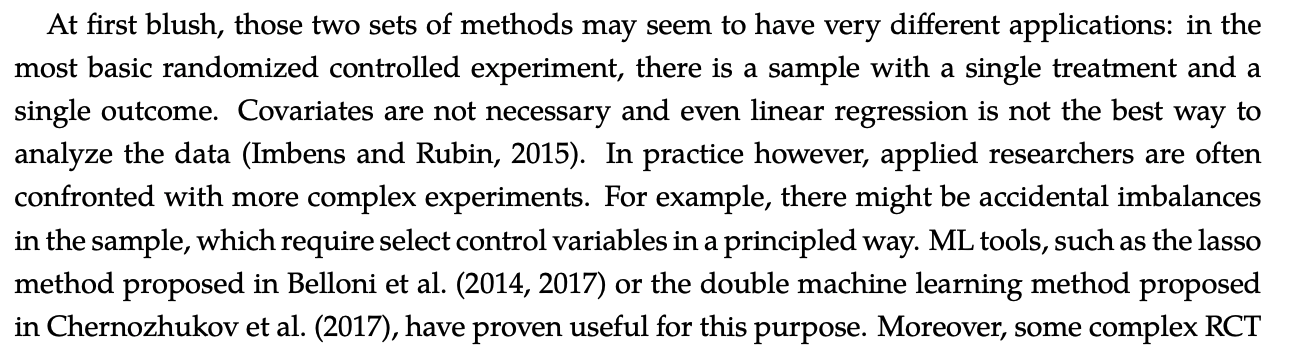
\includegraphics[width=\linewidth]{images/duflo_chernozhukov_ECMA.png}
  
  \begin{itemize}
  \item   Subsequent discussion regards \emph{subgroup analysis} -- a topic
    for our ML discussion at the end of the course!
    \begin{itemize}
    \item In essence, what if you have lots of treatment combinations /
      groups?
    \end{itemize}
  \end{itemize}
\end{frame}

\begin{frame}{The DML (Double/De-biased) Machine Learning Cookbook}
  $$Y_{i} = D_{i}\tau + g_{0}(X_{i}) + U_{i}, \qquad D_{i}, X_{i} \text{ are demeaned}$$  
  \begin{wideitemize}
  \item Will first outline the approach, then we can discuss details
  \item Key ingredients / assumptions:
    \begin{enumerate}
    \item \emph{Sparsity}; estimation error in $g_{0}$ is orthogonal
      to the moments that help estimate $D_{i}$
    \item Oracle condition is \emph{not} assumed
    \item Sample splitting; account for the overfitting bias from
      high-dimensional approaches
    \end{enumerate}
  \item Start with a ``naive'' approach
    \begin{enumerate}
    \item Split the sample in half
    \item Estimate $\hat{g}_{0}$ using one half of the sample using the regression
    \item Use this estimate $\hat{g}_{0}$ in the second half of the sample to construct:
      $$\hat{\tau} = \left(n^{-1}\sum_{i}D^{2}_{i}\right)^{-1}\left(n^{-1}\sum_{i}D_{i}(Y_{i} - \hat{g}(X_{i})\right)$$      
    \end{enumerate}
  \end{wideitemize}
\end{frame}

\begin{frame}{The DML (Double/De-biased) Machine Learning Cookbook}
  $$\hat{\tau} = \left(n^{-1}\sum_{i}D^{2}_{i}\right)^{-1}\left(n^{-1}\sum_{i}D_{i}(Y_{i} - \hat{g}(X_{i})\right)$$
  \begin{wideitemize}
  \item What happens here? If $D_{i} = m(X_{i}) + V_{i}$, and $m$ is a
    nontrivial function, then $|\sqrt{n}(\hat{\tau} - \tau)| \rightarrow \infty$
  \item Why?
    \begin{align*}
      \sqrt{n}(\hat{\tau} - \tau) &= \left(n^{-1}\sum_{i}D^{2}_{i}\right)^{-1}\left(n^{-1/2}\sum_{i}D_{i}U_{i}\right) \\
      &+ \underbrace{\left(n^{-1}\sum_{i}D^{2}_{i}\right)^{-1}\left(n^{-1/2}\sum_{i}D_{i}(g_{0} - \hat{g}_{0})\right)}_{\text{This term can blow up}}
      \end{align*}
  \end{wideitemize}
\end{frame}

\begin{frame}{The DML (Double/De-biased) Machine Learning Cookbook}
  \begin{wideitemize}
  \item In a correctly specified RCT, this term shouldn't
    matter. However, in finite samples (or with issues with controls),
    this could create poor performance (e.g. imbalance in treatment)
    \begin{itemize}
    \item Belloni, Chernozhukov, and Hansen (2014) discuss results
      where you can use lasso to directly choose the relevant controls
    \item I don't encourage this approach in cases where you don't
      have a positive story for identification -- an exclusively
      data-driven approach to choosing your controls is challenging
      for causal inference
    \end{itemize}
  \item What's the solution? Double lasso! In this setting, we need to
    do Frisch-Waugh style orthogonalization. E.g., also estimate
    $\hat{m}(X_{i})$
    \begin{itemize}
    \item E.g. $\hat{V}_{i} = D_{i} - \hat{m}(X_{i})$  and then
  $$\hat{\tau} = \left(n^{-1}\sum_{i}\hat{V}_{i}D_{i}\right)^{-1}\left(n^{-1}\sum_{i}\hat{V}_{i}(Y_{i} - \hat{g}(X_{i})\right)$$      
    \end{itemize}
  \end{wideitemize}
\end{frame}

\begin{frame}{What are the pieces of the DML estimator?}
  \begin{wideitemize}
  \item Three pieces to this estimator in the limiting distribution
    \begin{enumerate}
    \item The standard distribution
    \item Regularization bias -- assumed to small
    \item Remainder term -- sample splitting helps here
    \end{enumerate}
  \item How does this estimator get around the Leeb and Potscher critique?
    \begin{itemize}
    \item Estimation is not about nailing every piece of $g(X_{i})$ or $m(X_{i})$
    \item Instead, uniformity in $\hat{\tau}$ is achieved by having
      the estimation error in $g$ and $m$ be \emph{orthogonal} to
      $\hat{\theta}$'s estimation
    \item The key crucial (untestable) assumption: sparsity
    \end{itemize}
  \item Chernozhukov and co-authors also emphasize that the sample
    splitting is very effective at ensuring that many types of data
    processes can be incorporated
    \begin{itemize}
    \item Can simply sample split many times and then average over the
      estimates
    \item This is not necessary if you make stronger assumptions
    \end{itemize}
\end{wideitemize}
\end{frame}
\begin{frame}{The DML (Double/De-biased) Machine Learning Cookbook}
  \begin{wideitemize}
  \item We'll now walk through a simple example of estimation
    following Belloni, Chernozhukov and Hansen (2014):
    \begin{itemize}
    \item A fully exogeneous binary treatment
    \item Set of controls
    \item Lasso estimation of $g(X)$ and $m(X)$
    \item No splitting
    \end{itemize}
  \item If you want a different estimator, consult
    Chernozhukov, Chetverikov, Demirer, Duflo, Hansen, Newey and
    Robins (2018)
  \end{wideitemize}
\end{frame}

\begin{frame}{Simple lasso approach w/o splitting}
  The approach, straight out of Belloni, Chernozukhov, and Hansen (2014)
  \begin{enumerate}
  \item Estimate lasso of $D_{i}$ on the control set $X$ and identify
    the controls selected by the procedure (don't lasso on the
    constant). Call this set of $X_{i}$ $I_{1}$
    \begin{itemize}
    \item Note -- choice of penalization term matters. Discussed in Appendix A of Belloni (2012)
    \item I just use the \texttt{rlasso} package in R, or \texttt{rlasso} in Stata (\texttt{lassopack})
    \end{itemize}
  \item Estimate lasso of $Y_{i}$ on the control set $X$ and identify
    the controls selected by the procedure (don't lasso on the
    constant). Call this set of $X_{i}$ $I_{2}$ 
  \item Rerun OLS with $D_{i}$ and the union of $I_{1}$ and $I_{2}$ as
    controls (you can add in other variables too if they're not too
    big)
  \item That's it! Interpret the coefficient on $D_{i}$ as you will
    \begin{itemize}
    \item Note from Wuthrich and Zhu (2020) -- can be finite sample
      issues. Make sure your results are robust to shifting your
      tuning parameters
    \end{itemize}
  \end{enumerate}
\end{frame}


\end{document}

